\documentclass[hyperref={pdfpagelabels=false},t,10pt]{beamer}
\usepackage[utf8]{inputenc}
\usepackage[english]{babel}
\usepackage[T1]{fontenc}
\usepackage[default,scale=.95]{opensans}
\usepackage{tikz}
\usepackage{graphicx}



\usetheme[cd2018]{tud}
\setbeamercolor{normal text}{fg=black}
\colorlet{alert}{cdblue}
\setbeamercolor{alerted text}{fg=cdblue}
\setbeamerfont{frametitle}{size=\Large,family=\sffamily,series=\sbseries}


\DeclareRobustCommand\sbseries{\fontseries{sb}\selectfont}
\DeclareTextFontCommand{\textsb}{\sbseries}


\title{IP = PSPACE}
\author[© author]{hello}
\institute{Technische Universit\"at Dresden}
\datecity{CONFERENCE}
\date{DATE}


\begin{document}

%%%% Uncomment the following line to set background image to main slide
%%%% (parameter sets transparency)
%\setbeamertemplate{tud background}[image/shaded]{background.jpg}{0.5}
\addtocounter{framenumber}{-1}
\maketitle
\begin{frame}
  \frametitle{Content}
  \begin{itemize}
    \item What is IP?
    \item Short idea for $PSPACE \in IP$
    \item Arithmetization
    \item Introducing the protocol 
    \item Problems within the protocol and solutions
    \item Some protocol examples
    \item Correctness
  \end{itemize}
\end{frame}

\begin{frame}
  \frametitle{PSPACE $\subseteq$ IP}
  For this inclusion, we use a well known PSPACE-complete problem, namely True-QBF
  \pause
  \begin{itemize}
  \item QBF-Truth is the set of all valid quantified boolean formulas without free variables and for any variable p we have $p\in \{0,1\}$
  \pause
  \item $\forall x \exists y \, (x \lor y)$, $\exists x \exists y \neg(x \land y)$
  \pause
  \item $\mbox{QBF-Truth}_{NNF}$ (abbrev. with QBF') is QBF-Truth but negations are only applied on variables
  \item $\exists x \exists y \neg(x\land y)$ is not in NNF but $\exists x \exists y (\neg x \lor \neg y)$
  \pause
  \item $\mbox{QBF} \leq^P_m \mbox{QBF-Truth}_{NNF}$ can be easily done by the verifier 
  \item it suffices to show QBF' $\in$ IP because we can reduce any problem in PSPACE to QBF in polynomial time \newline \newline
  How do we find an algorithm for QBF' s.t it satisfies the IP conditions?

  \end{itemize}
\end{frame}

\begin{frame}
  \frametitle{Arithmetization}
  The prover has to convince the verifier that the formula is valid but in case of 
  an invalid formula it should reject with high probability (for all prover) \newline \pause

  \begin{itemize}
    \item The idea is to arithmetize the formula \pause
    \item $x \land y$ becomes x*y
    \item $x \lor y$ becomes x+y
    \item $\neg x$ becomes 1-x \pause
  \end{itemize}
    \begin{tabular}{|c|c|c|c|c|}
      \hline
      x & y & $x\land y = x*y$& $x\land y = x+y $ &$\neg (x\land y) = 1- (x * y)$ \\ 
      \hline
      0 & 0 & 0 & 0 & 1\\ 
      0 & 1 & 0 & 1 & 1\\
      1 & 0 & 0 & 1 & 1\\
      1 & 1 & 1 & 2 & 0\\ 
    \end{tabular}
    $$\phi(x_1,x_2,...,x_n) = 1 \Leftrightarrow \phi_{arith}(x_1,x_2,...,x_n) > 0$$
\end{frame}

\begin{frame}
  \frametitle{Arithmetization}
  How do we arithmetize $\forall$ and $\exists$ ?  \newline
  \pause 

  \begin{itemize}
    \item $\forall x \, \phi$ becomes $a_0 * a_1$ where $a_0 = \phi[x := 0]$ and $a_1 = \phi[x := 1]$ 
    \pause
    \item $\exists x \, \phi$ becomes $a_0 + a_1$ where $a_0 = \phi[x := 0]$ and $a_1 = \phi[x := 1]$  
    \pause
  \end{itemize}
  Example : $\phi = \forall x \exists y \, \neg (x \land y)$ \newline \pause 
  Arithmetize : $\neg (x \land y) \, \xrightarrow{arith.} 1-(x * y) \xrightarrow{\exists arith.} \sum_{y \in \{0,1\}}^{} 1-(x*y) \xrightarrow{\forall arith.}$ \pause \newline 
  $\prod_{x \in \{0,1\}}^{} \sum_{y \in \{0,1\}} 1- (x*y) = \phi_{arith}$ \newline

  \begin{itemize}
    \item $\phi_{arith} = 2$ \pause
    \item If $\phi$ is true then $\phi_{arith} > 0$
    \item If $\phi$ is false then $\phi_{arith} = 0$ \pause
    \item This can be shown by structural induction 
  \end{itemize}
\end{frame}

\begin{frame}
  \frametitle{Arithmetization}
  \begin{itemize}
    \item $\phi = x$. If $\phi$ is true then $\phi_{arith} = 1$ and if $\phi $ is true then $\phi_{arith} = 0$
    \item $\phi = \neg x$ is the same but turned around \pause
    \item Suppose $\phi_1$ and $\phi_2$ are true, that means $\phi_{1arith} > 0$ and $\phi_{2arith} > 0$ \newline(it's similar for the other case)\pause
    \item $\phi_1 \land \phi_2$, $\phi_1 \lor \phi_2$ also holds
    \item For $\forall \, \phi_1$, we have by induction that $\phi_1[x := 0], \phi_1[x := 1]$ is true, so the multiplication of two positive value is positive (same for $\exists \phi_1$)
  \end{itemize}
\end{frame}

\begin{frame}
  \frametitle{Protocol-Problem}
  How do we start the communication between prover and verifier? \pause

  \begin{itemize}
    \item On input <$\phi$>, the prove sends a value c>0 to the verifier and tries to convince that c is the arithmetic value of $\phi$ \newline (Remember : the verifier can not calculate its value by itself because it could be double exponential) \pause
    \item Problem : the value could be exponential but the verifier has only polynomial time \pause
  \end{itemize}

  $\phi = \forall x_1 ... \forall x_m \exists y \exists z. (y \lor z)$. What is $\phi_{arith}$? We caluclate it step by step. \pause
  Let $\phi' = \exists y \exists z (y \lor z)$. Then $\phi'_{arith} = \sum_{y \{0,1\}}^{} \sum_{z \{0,1\}^{}} y + z = 4$ \pause
  $\phi_{arith} = \prod_{x_1 \in \{0,1\}}^{}... \prod_{x_m \in \{0,1\}}^{} \phi'_{arith} = 4^{2^{m}}$ \newline
  \begin{itemize}
    \item It holds that for formula $\phi$ with string length n : $\phi_{arith} \leq 2^{2^{n}}$
    \item  We solve this problem by using modulo with a suitable value
  \end{itemize}
\end{frame}

\begin{frame}
  \frametitle{Protocol-Problem}
  \begin{itemize}
    \item Pick a value $k \geq 2^n$ with two conditions : 
    \item k must be presentable in linear many bits \pause
    \item the calculation mod k must preserve ">0" for valid and "=0" for invalid formulas
    \item Number Theory Theorem : for any $a \leq 2^{2^{n}}, a>0$, there exist a prime number $k \in [2^n, 2^{3n}]$ s.t $a \not\equiv 0 $ (mod k)
  \end{itemize}
\end{frame}

\begin{frame}
  \frametitle{Protocol continued}
  \begin{itemize}
    \item Prover sends value c, prime number k and a proof b for the prime number property (it is possible to give a polynomial proof) \pause
    \item Verifier check c>0, $k \in [2^n, 2^{3n}]$ and b is a correct proof for prime property 
  \end{itemize}
  Even if k and b are correct, the verifier stays sceptical about c. \pause

  \begin{itemize}
    \item If $\phi = \phi_1 \land \phi_2 $, then ask prover to send $a_1$ and $a_2$ and check $c = a_1 * a_2$. If it's true then ask the prover to prove that the of $\phi_1$ is $a_1$ and $\phi_2$ is $a_2$
    \item For $\phi = \phi_1 \lor \phi_2$, we ask for $a_1$ and $a_2$ s.t c = $a_1 + a_2$ \pause
    \item In case $\phi = \forall x \phi_1$ we asked for a polynomial p(x) that represents the arithmetic presentation of $\phi_1$ where x is free and we check c = p(0) * p(1)
    \item If it is true, the verifier sends randomly a number d between $\{0,..., k-1\} = GF(K)$ and caluclate p(d). Now the verifier expects the prover to prove the value of $\phi_1[x := d]$ is p(d)
    \item The same process happens when we have $\phi = \exists \phi_1$, but we check $c = p(0) + p(1)$
  \end{itemize}
  
\end{frame}

\begin{frame}
\frametitle{Protocol continue}
\begin{itemize}
  \item When every variable got a number in GF(K), say $y_1, ..., y_n$ the verifier calculates $\phi_{arith}(y_1,...,y_n)$ and accept if its equal to $q(y_1,...,y_n)$ (last polynomial sent by prover) else reject
\end{itemize}
\end{frame}


\begin{frame}
  \frametitle{Example}
  $\phi = \forall x \exists y (\neg x \lor y) \land \exists z \exists w \, (z \lor w) $ \newline \newline
  $\phi_{arith} = \underbrace{(\prod_{x}^{} \prod_{y}^{} (1-x) + y )}_{\phi_{1arith}} * \underbrace{(\sum_{z}^{} \sum_{w}^{} z + w)}_{\phi_{2arith}}$ \, \,   $x,y,z,w \in \{0,1\}$ \pause
  \newline
  %\hspace*{1.3cm} Prover \hspace{6.8cm} Verifier \newline \newline
  \hspace*{0cm}
  \begin{tikzpicture}
    \node at (-2,0.5) {Prover};
    \node at (8,0.5) {Verifier};
  \draw[->] (0,0) -- (6,0) node[midway, above] {c=8,k=11,b};
  \node[text width=5cm, align=left] at (9,0) {check c>0, 8, b}; \pause
  \draw[<-] (0,-1) -- (6,-1) node[midway, above] {asks for $a_1 = \phi_1 \mbox{ and } a_2 = \phi_2$};
  \draw[->] (0,-2) -- (6,-2) node[midway, above] {sends $a_1 = 2$, $a_2 = 4$};
  \node[text width=5cm, align=left] at (9,-2) {check $c = a_1 * a_2$};
  \draw[<-] (0,-3) -- (6,-3) node[midway, above] {prove $a_1 = \phi_1, a_2 =\phi_2$}; \pause
    \draw[<-] (0,-3) -- (6,-3) node[midway, below] {send me $p_1(x)$ for $\phi_1$ and $p_2(x)$ for $\phi_2$};
  \end{tikzpicture}

\end{frame}

\begin{frame}
   \hspace*{0cm}
  \frametitle{Example continue}
  \begin{tikzpicture}
    \node at (-2,0.5) {Prover};
    \node at (8,0.5) {Verifier};
    \node[text width=1.5cm, align=left] at (-2,-0.5) {\small calculate $\phi_{1arith}(x)$, $\phi_{2arith}(z)$}; 
    \draw[->] (0,-0.5) -- (6,-0.5) node[midway, above] {\small sends $p_1(x) = \phi_{1arith}(x)$, $\phi_{2arith}(z)$};
    \draw[->] (0,-0.5) -- (6,-0.5) node[midway, below] {\small $p_1(x) = \prod_{y}^{}(1-x)+y = x^2-3x+2$};
    \node[text width=3.5cm, align=left] at (8,-0.5) {\scriptsize check $a_1=p_1(0)*p_1(1)$};
    \node[text width=3.5cm, align=left] at (8,-0.9) {\scriptsize check $a_2=p_2(0)+p_2(1)$}; \pause 

    \node[text width=3.5cm, align=left] at (8,-2.5) {\scriptsize Choose randomly $d,g \in GF(k)$,say d=2,g=3};
    \draw[<-] (0,-2.5) -- (6,-2.5) node[midway, above] {\small sends $p_1(d) = 0, p_2(g) = 7$};
    \draw[<-] (0,-2.5) -- (6,-2.5) node[midway, below] {\small ask for $p'_1(d,y), p'_2(g,w) $}; \pause
    \draw[->] (0,-4.5) -- (6,-4.5) node[midway, above] {\small sends $p'_1(d,y) = \phi_{1arith}(d,y)$};
    \draw[->] (0,-4.5) -- (6,-4.5) node[midway, below] {\small sends $p'_2(g,w) = \phi_{2arith}(g,w)$};
    \node[text width=3.5cm, align=left] at (8,-4.5) {\scriptsize $p'_1(d,0)*p'_1(d,1)=p_1(d)$};  
    \node[text width=3.5cm, align=left] at (8,-4.9) {\scriptsize $p'_2(g,0)*p'_2(g,1)=p_2(g)$}; 
    \node[text width=3.5cm, align=left] at (8,-5.3) {\scriptsize Choose c,k $\in$ GF(k)}; \pause
  \end{tikzpicture} 
  \pause
    \only<5->{ % Replace 5 with the slide number where it should appear
    \vspace{0.5cm}
    \text{The verifier check $\phi_{arith}(d,c,g,k) = p'_1(d,c) * p'_2(g,k)$. It accepts.}
  }
\end{frame}

\begin{frame}
  \hspace*{0cm}
  \frametitle{Next Example}
  $\phi = \forall x \exists y \,x \land y  \xrightarrow{arith.} \phi_{arith} = \prod_{x}^{} \sum_{y}^{} x*y$ \pause \newline \newline
  Prover can not tell the truth because the verifier would reject instantly.
  \begin{tikzpicture}
    \node at (-2,-0.5) {Prover};
    \node at (8,-0.5) {Verifier}; \pause  
    \draw[->] (0,-0.5) -- (6,-0.5) node[midway, above] {c= 3, p = 131, b};
    \node[text width=5cm, align=left] at (9,-1) {\small check c>0, 131, b};
    \draw[<-] (0,-1.5) -- (6,-1.5) node[midway, above] {asks for $p_1(x)$}; \pause
    \draw[->] (0,-2.5) -- (6,-2.5) node[midway, above] {sends $p_1(x) = 2x + x$};
    \draw[->] (0,-2.5) -- (6,-2.5) node[midway, below] {\small prover has to lie};
    \node[text width=5cm, align=left] at (9,-2.5) {\scriptsize check $p_1(0) * p_1(1) = c$}; \pause
    \node[text width=5cm, align=left] at (9,-3) {\scriptsize choose $d\in GF(p)$};
    \draw[<-] (0,-3.5) -- (6,-3.5) node[midway, above] {\small sends $p_1(d)$};
    \draw[<-] (0,-3.5) -- (6,-3.5) node[midway, below] {\scriptsize If $\phi_{arith}(d)= p_1(d=3) = 7$ then we lost. Chances should be low}; \pause
    \draw[->] (0,-4.5) -- (6,-4.5) node[midway, above] {\small sends $p'_1(d,y) = 7*y$};
    \node[text width=3.5cm, align=left] at (8,-4.5) {\scriptsize check $p'_1(d,0) + p'_1(d,1) = p_1(d)$. Chooses g = 4};
  \end{tikzpicture}
  \only<5->{ % Replace 5 with the slide number where it should appear
    \vspace{0.5cm}
    \text{The verifier check $\phi_{arith}(d,g) = p'_1(d,g)$. $12\neq 28$. Verfier rejects.}
  } 

\end{frame}

\begin{frame}
  \frametitle{Simple QBF}
\begin{itemize}
  \item Problem : Polynomial could be exponential. The verifier can not verfying it in polynomial time. \pause
  \item Example : $\phi = \forall x_1, ... , \forall x_m (x_1 \lor ... \lor x_m) \xrightarrow{arith \phi(x_1)} \phi_{arith}(x) = \prod_{x_2}^{} ...\prod_{x_m}^{}\, (x_1 +x_2+ ...+ x_m) \rightarrow deg(\phi_{arith}(x)) \leq 2^{m-1}$ \pause
  \item A QBF $\phi$ is called simple, if any occurence of a variable is seperated by at most one universal quantifier from its point of quantification.
  \item Example : $\forall x_1 \forall x_2 \exists x_3$ $[(x_1 \lor x_2) \land \forall x_4 (x_2 \lor x_3 \lor x_4)]$
  \item Counterexample : $\forall x_1 \forall x_2 [(x_1 \lor x_2) \land \forall x_3 (\neg x_1 \lor x_3)]$ \pause
  \item We can reduce any QBF formula into a Simple QBF in polynomial time
  \item Let $\phi = ... Qx_i...\forall x_j \psi(x_i)$ where $Q \in \{\forall, \exists\}$ and $\forall x_j$ is the first universal quantifier after $Q_{xi}$. We transform $\phi$ as follows :
  $$\phi' = ... Qx_i ... \forall x_j\exists x_i' (x_i \leftrightarrow x_i') \land \psi(x_i')$$
\end{itemize}
\end{frame}


\begin{frame}
  \frametitle{Correctness}
  \begin{itemize}
    \item Example : $\exists x (\forall y \forall z (x \lor (y \lor z))) \land (\forall u (u \lor x))$
    \item Reduced : $\exists x (\forall y \exists x'  (x \leftrightarrow x') \land \forall z(x' \lor (y \lor z))) \land (\forall u (u \lor x))$
    \item If $\phi$ is a simple QBF formula of length n,and p(x) be a polynomial of $\phi_{arith}$. Then $deg(p(x) \leq 2^n)$. This can be shown by induction. \pause
  \end{itemize}
  Now we check for the correctness of the protocol

  \begin{itemize}
    \item If $\phi$ is true, a truthful Prover can ensure that V accepts \pause
    \item If $\phi$ is false, the chance that V accepts is very small \pause
    \item We use "Schwartz-Zippel" lemma. Let p be a non-zero multivariate polynomial $p(x_1,...,x_m)$ with degree $\leq d$ and S a finite set of integers.
    If $a_1,..., a_m$ a chosen randomly independently and uniformly from S, then $$Pr[p(a_1,...,a_m)= 0] \leq \frac{d}{|S|}$$ \pause
    \item Prover sends wrong polynomial $p \neq h =\phi_{arith}$ in the i-th round. Verifier chooses randomly $c\in GF(p)$ where $p\geq 2^n$. Furthermore we have $deg(g-h) \leq 2n$.
    Then $Pr[p(c) = h(c)] = \mbox{Pr[Error i-th round]} \leq \frac{2n}{2^n}$.
  \end{itemize}
\end{frame}

\begin{frame}
  \frametitle{Correctness continue}
  \begin{itemize}
    \item That means Pr[No Error in i-th round]$\geq 1- \frac{2n}{2^n}$
    \item Because random number are chosen independently, and after $m \leq n$ rounds, we have : 
    $$Pr[Error] = 1 - Pr[\mbox{No Error}] = 1- \prod_{i=1}^{m} Pr[\mbox{No Error in i-th round}]$$
    $$ \leq (1-(1-\frac{2n}{2^n}))^n$$ \newline
    \item  The last approximation is true because : $\prod_{i=1}^{m} Pr[\mbox{no error in i-th round}] \geq (1-\frac{2n}{2^n})^m \geq (1- \frac{2n}{2^n})^n$
  \end{itemize}
\end{frame}

\begin{frame}
  \begin{figure}[h]
    \centering
    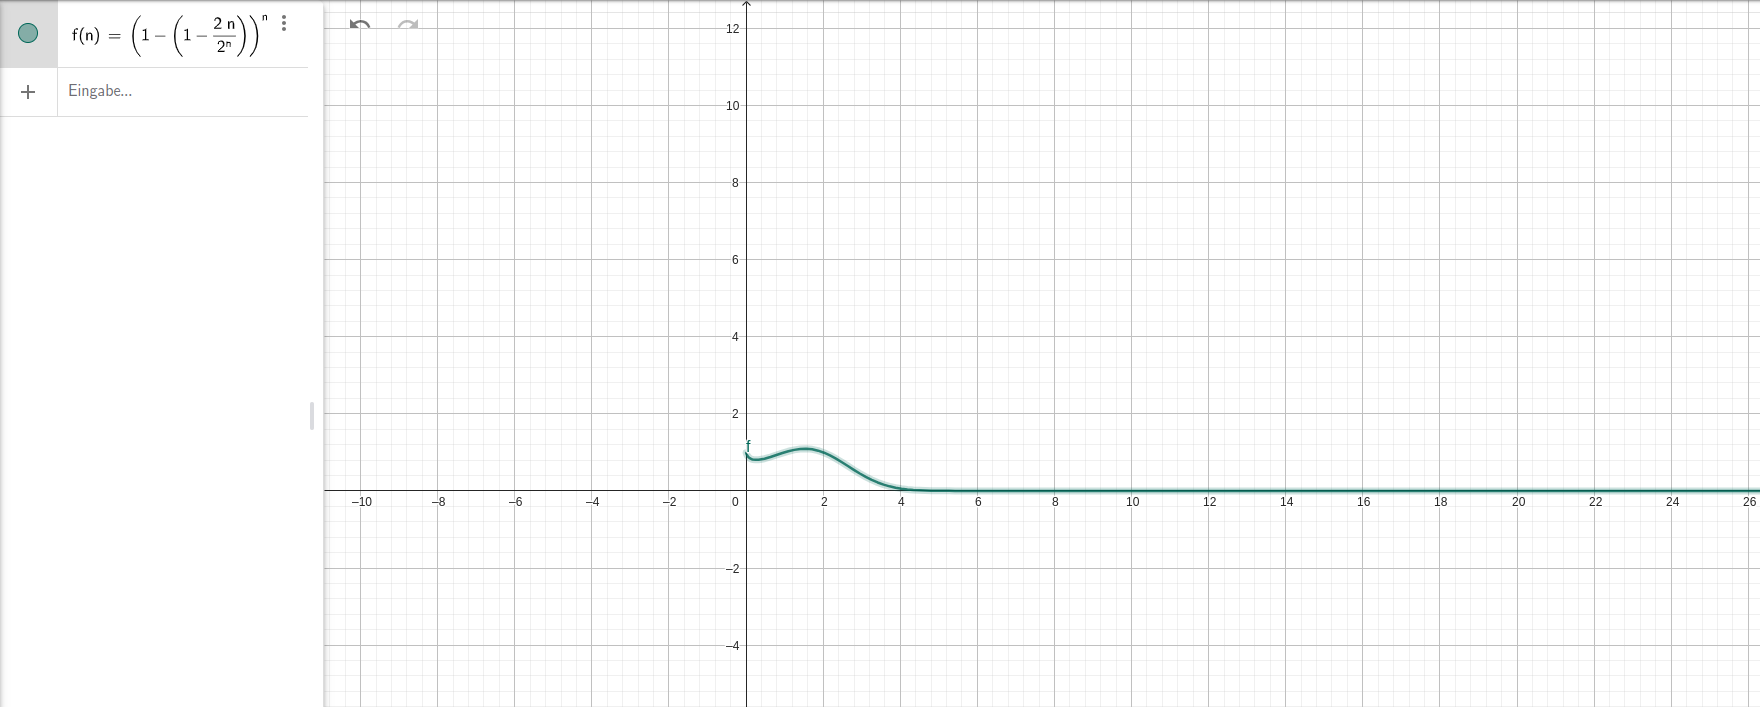
\includegraphics[scale= 0.25]{Copy.png}
    \caption{$n \rightarrow \infty$}
  \end{figure}
\end{frame}
\end{document}
